\chapter{需求建模 }
\section{数据流图}
\subsection{顶层数据流图}
\begin{figure}[h]
	\centering
	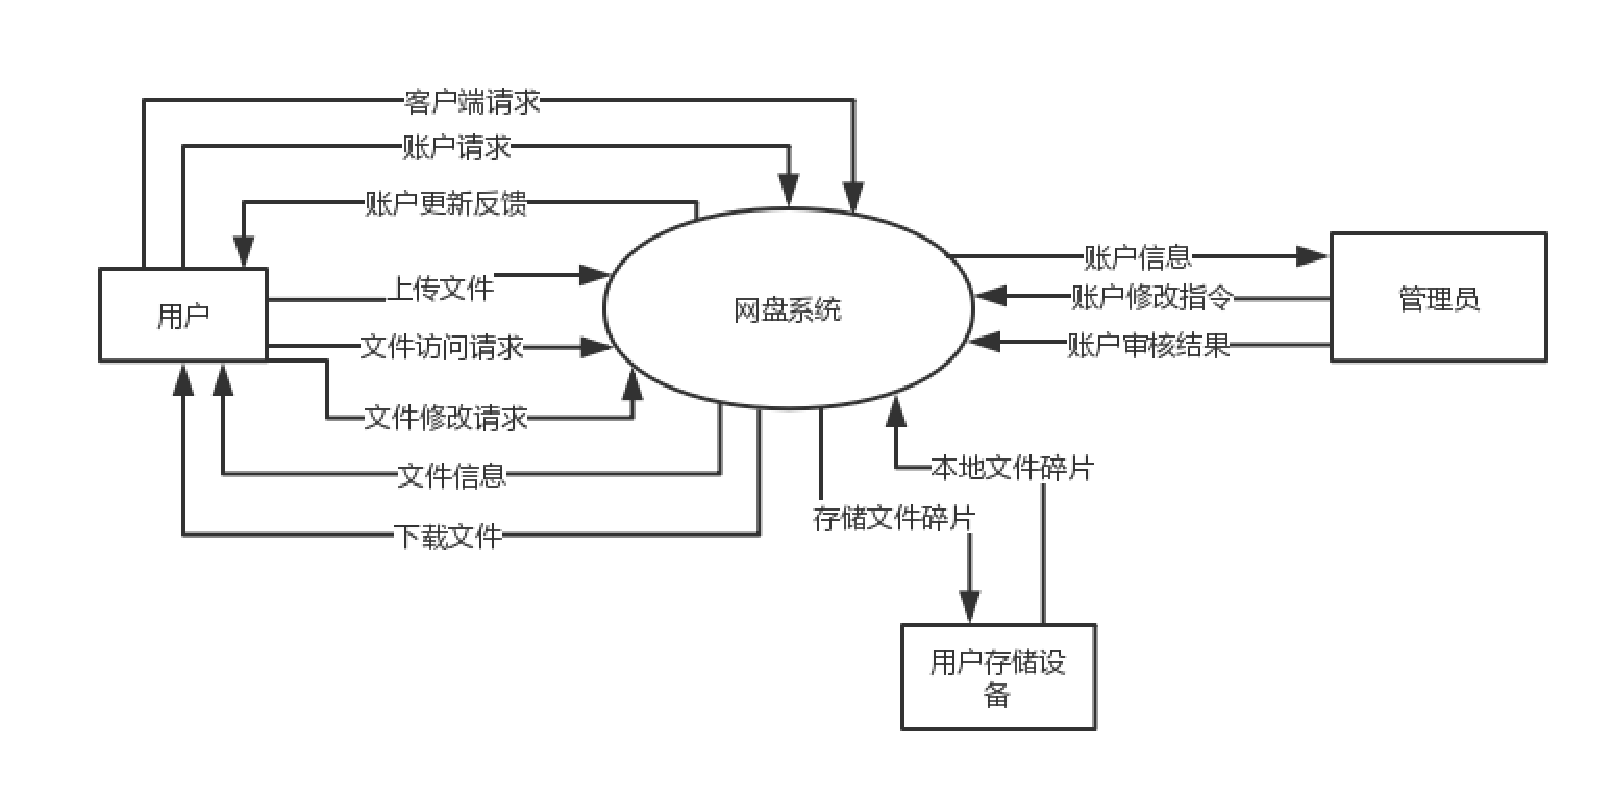
\includegraphics[width=12cm]{top_level_DFD}
	\caption{top level DFD} \label{fig:figure2}
\end{figure}

\subsection{0层数据流图}
\begin{figure}[h]
	\centering
	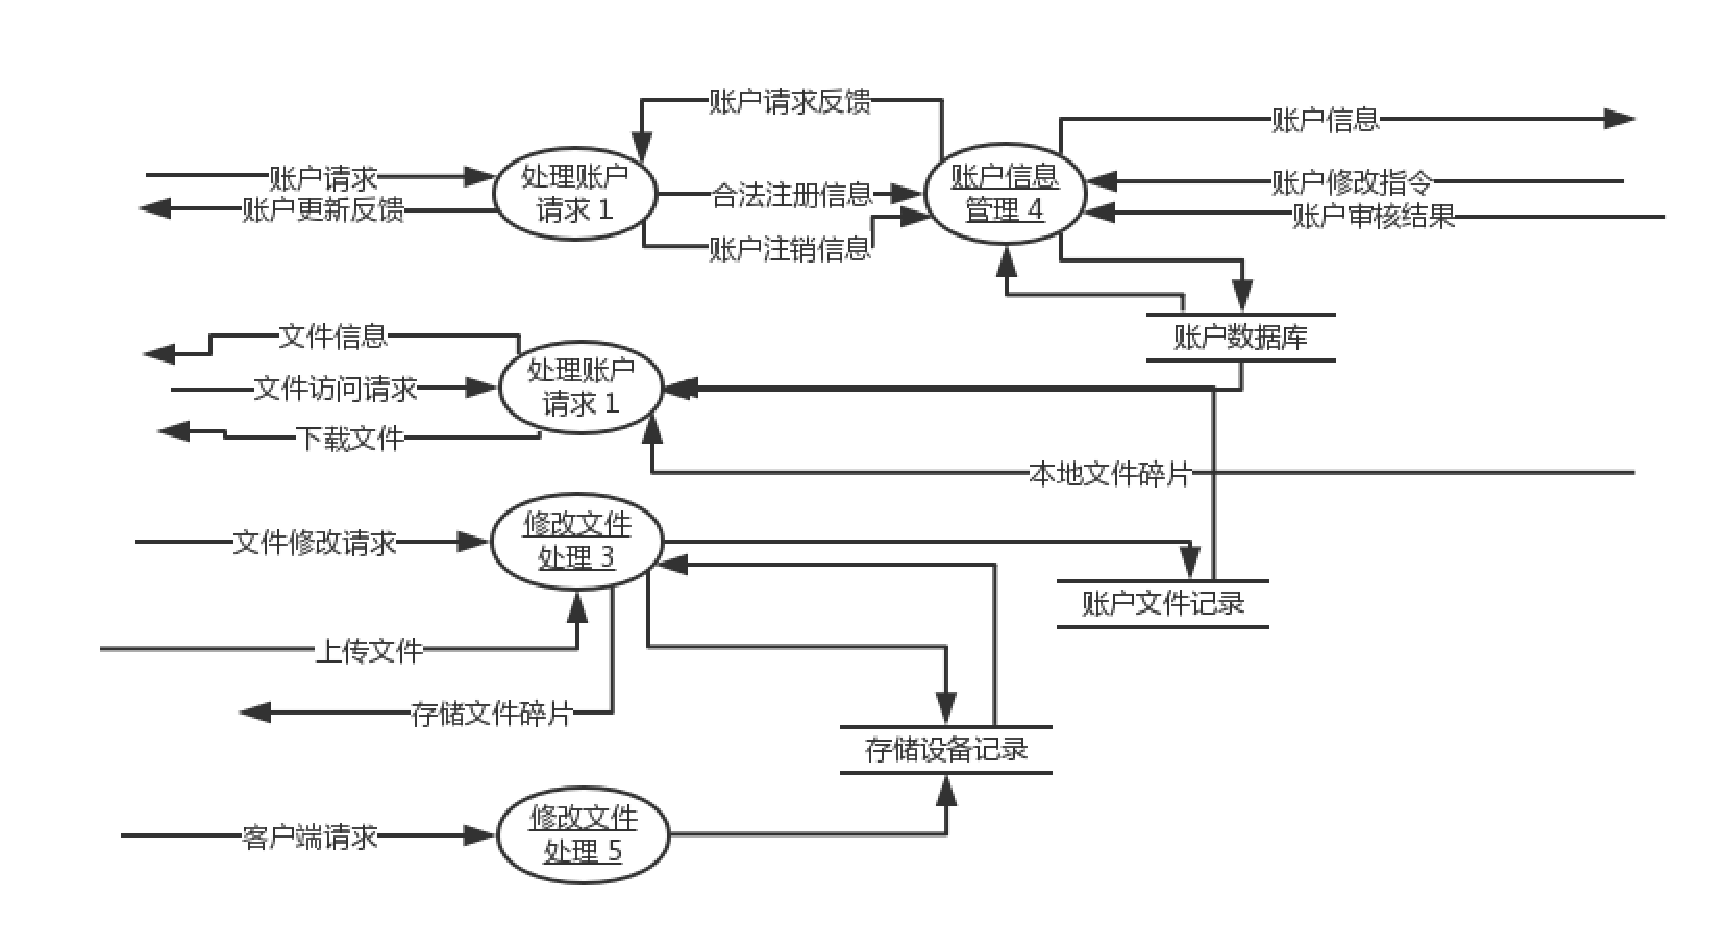
\includegraphics[width=13cm]{0_level_DFD}
	\caption{0 level DFD} \label{fig:figure3}
\end{figure}

\subsection{1层数据流图}
\begin{figure}[h]
	\centering
	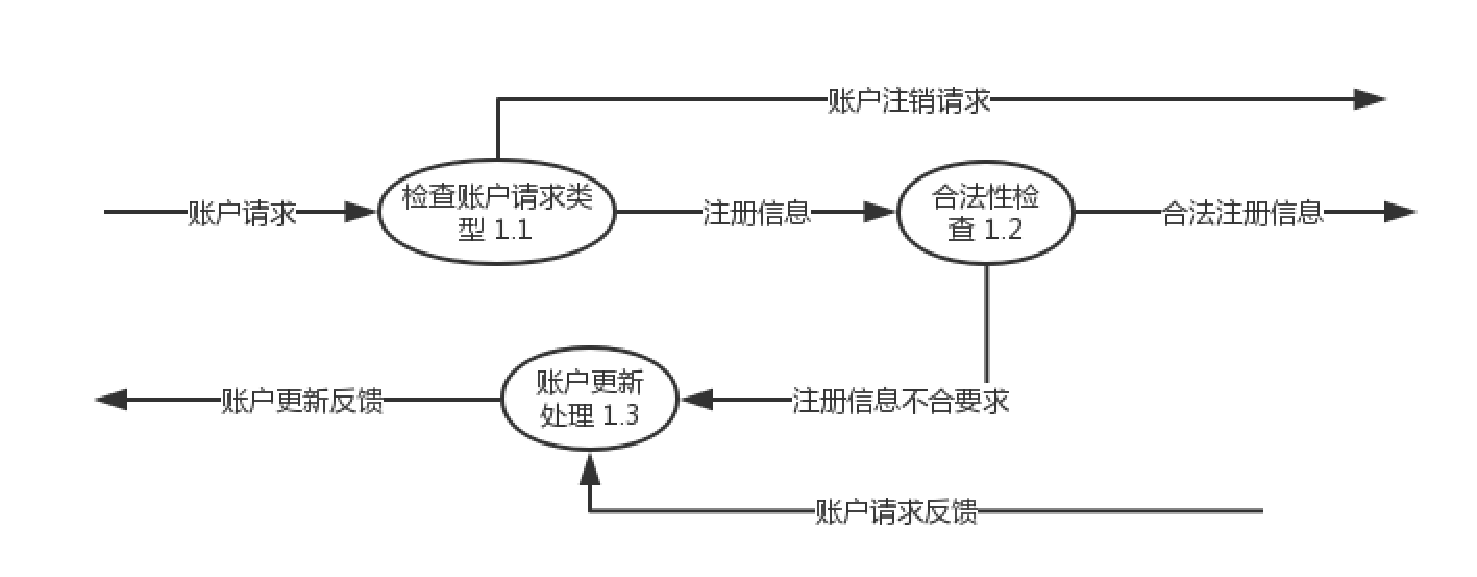
\includegraphics[width=13cm]{1_level_DFD_picture1}
	\caption{1 level DFD picture1} \label{fig:figure4}
	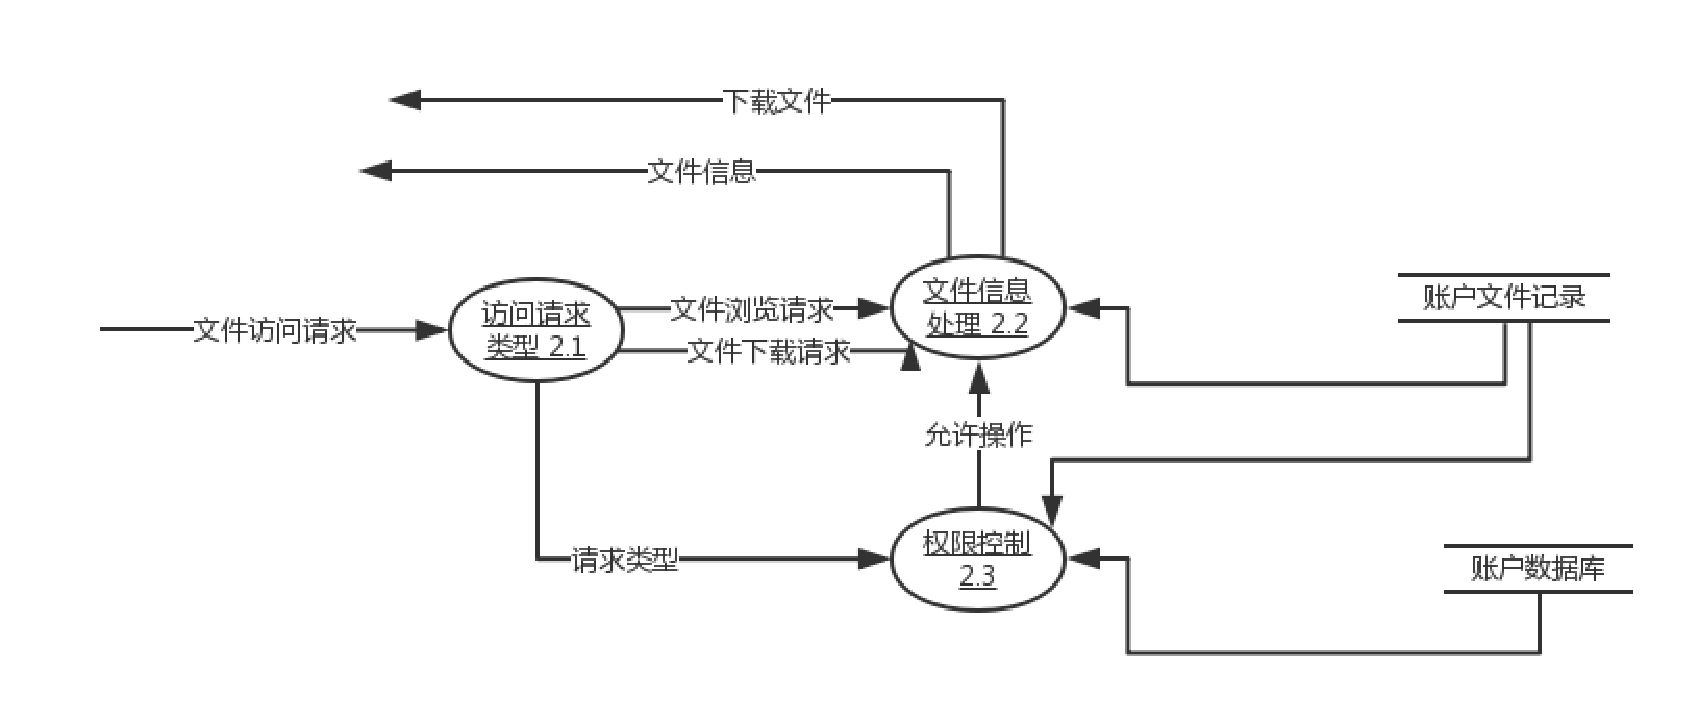
\includegraphics[width=13cm]{1_level_DFD_picture2}
	\caption{top level DFD picture2} \label{fig:figure5}
\end{figure}
\begin{figure}[h]
	\centering
	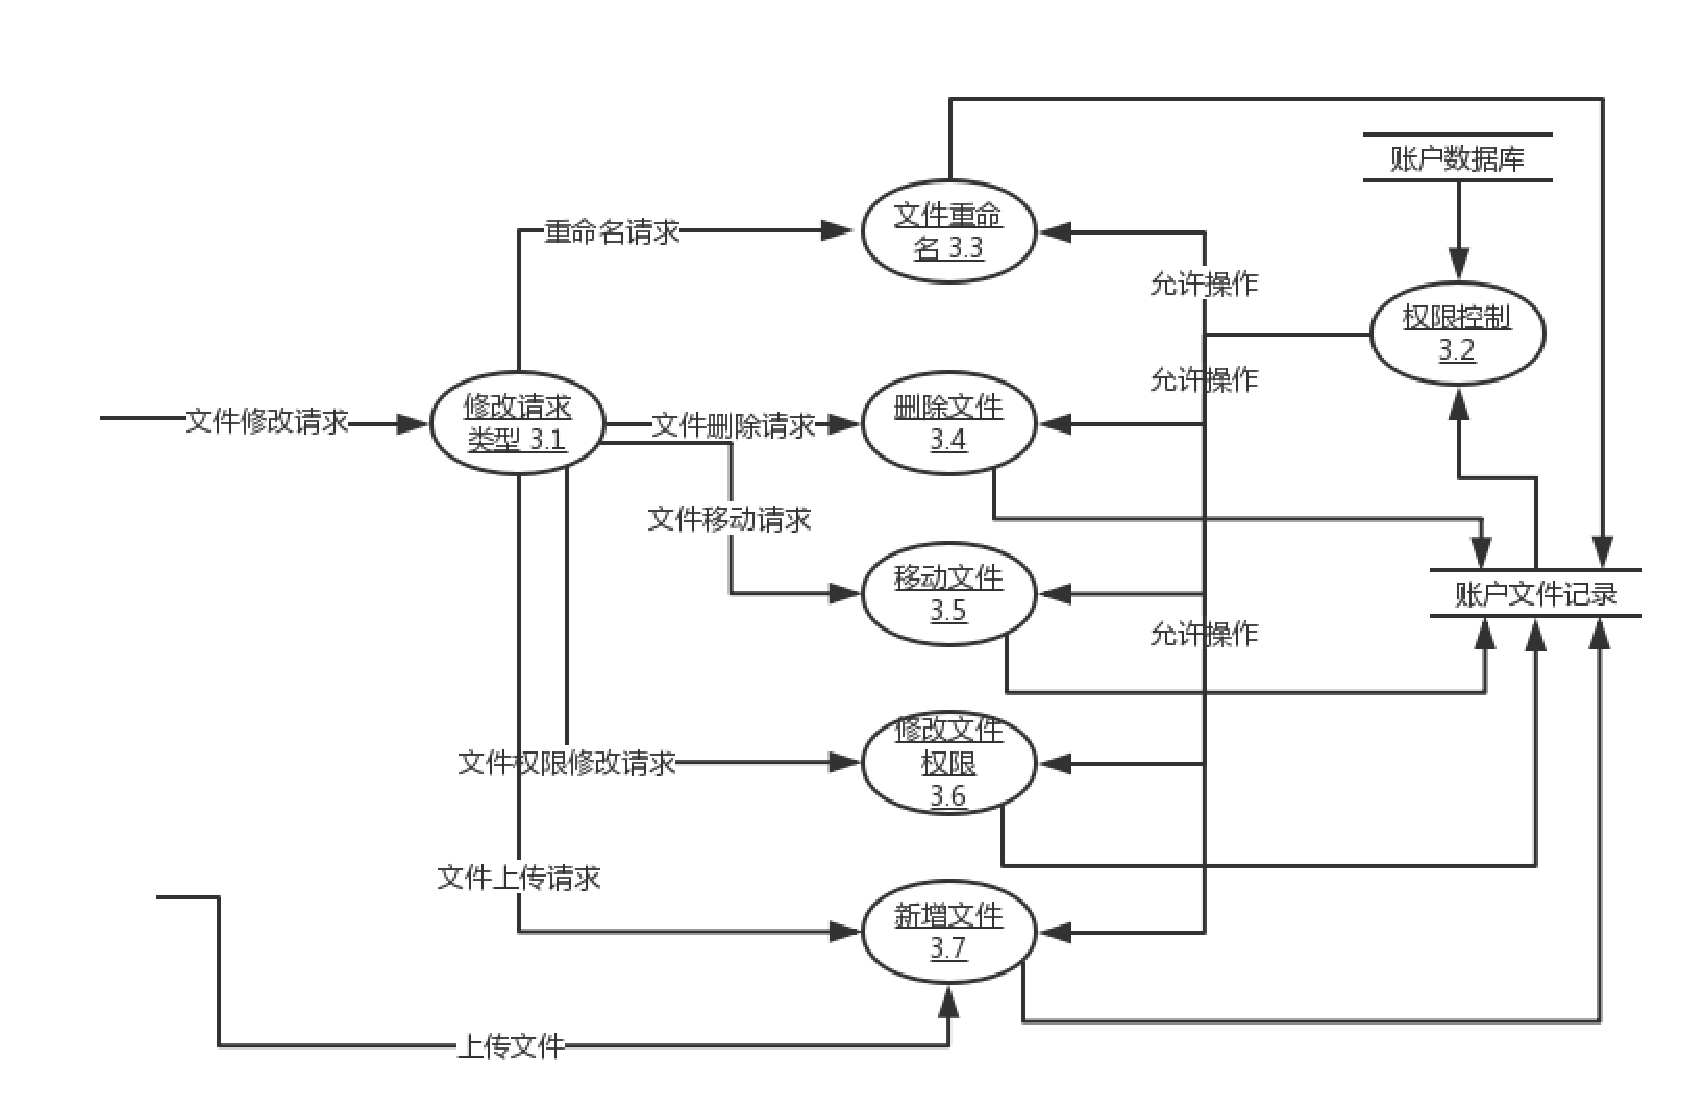
\includegraphics[width=12cm]{1_level_DFD_picture3}
	\caption{top level DFD picture3} \label{fig:figure6}
	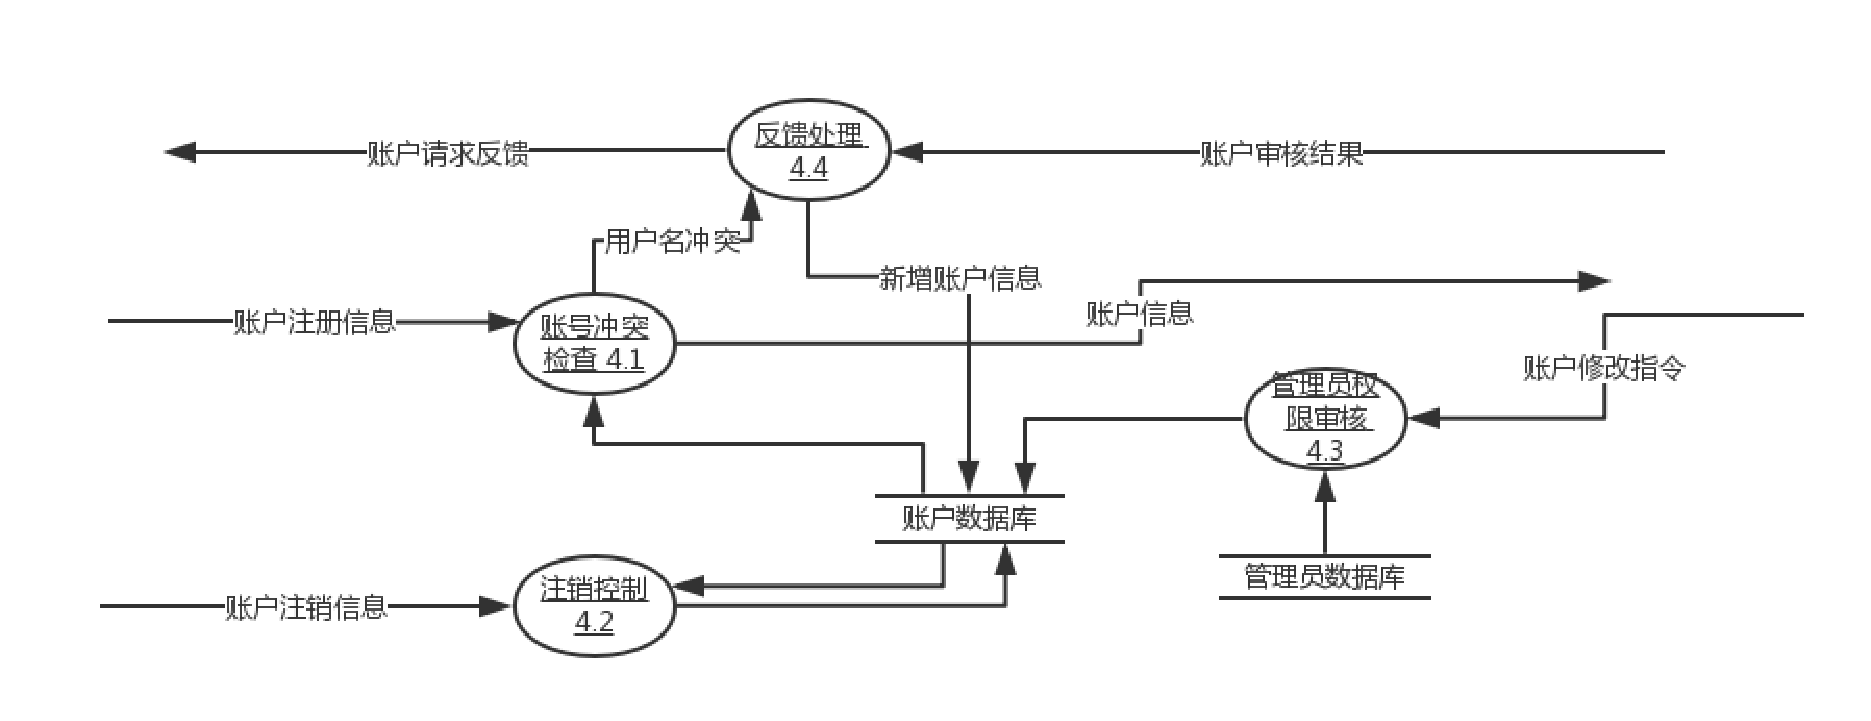
\includegraphics[width=12cm]{1_level_DFD_picture4}
	\caption{top level DFD picture4} \label{fig:figure7}
	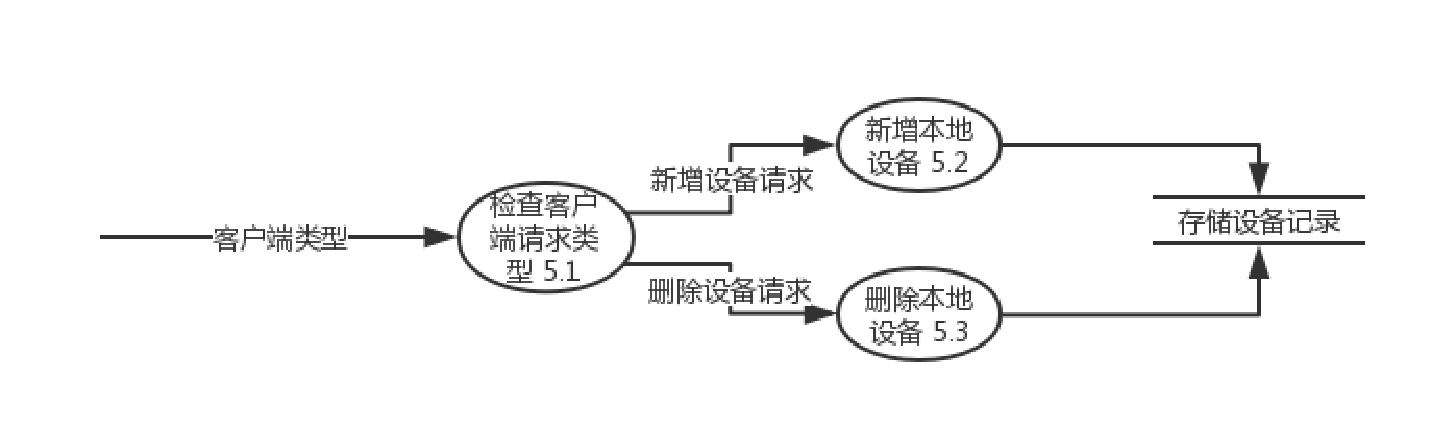
\includegraphics[width=12cm]{1_level_DFD_picture5}
	\caption{top level DFD picture5} \label{fig:figure8}
\end{figure}

\section{数据字典}
\subsection{数据流说明}
\subsubsection{客户端请求}
用户客户端发送的请求,包括增加本地设备和删除本地设备。

\subsubsection{账户请求}
用户对账号操作的请求,包括注册账号和注销账号。

\subsubsection{账户更新反馈}
系统对用户账户请求的处理结果的反馈信息。失败时包含失败原因,成功时提示用户跳转到登陆界面。

\subsubsection{上传文件}
用户上传的文件,须在上传文件请求通过后提供。

\subsubsection{文件访问请求}
用户对网盘上文件的读操作,包括查看文件目录和下载文件。

\subsubsection{文件修改请求}
用户对网盘上的文件的写操作,包括文件上传、文件移动、文件删除、文件重命名等。

\subsubsection{文件信息}
系统对用户的访问请求的反馈,包含该用户在网盘上的存储信息。

\subsubsection{下载文件}
用户从网盘上下载的文件。

\subsubsection{账户信息}
系统提供用户账户信息给管理员。此数据流可能在用户注册时产生,也可能在管理员查询用户状态时产生。

\subsubsection{账户修改指令}
管理员对系统中用户账户的修改操作,包括删除账户、密码重置、修改用户存储上限。

\subsubsection{账户审核结果}
管理员对用户注册的审核结果。

\subsubsection{存储文件碎片}
由系统分配给存储设备进行分布式存储的文件碎片。

\subsubsection{本地文件碎片}
存储设备上传的文件碎片。

\subsubsection{账户请求反馈}
账户注册或注销请求的处理结果反馈。注册失败时包含失败原因(用户名冲突、管理员拒绝)。

\subsubsection{合法注册信息}
用户注册时提交的信息,已经过合法性检查,符合注册要求,但为检查账号冲突。

\subsubsection{账户注销信息}
用户注销账号时提交的信息

\subsubsection{注册信息}
用户提供的注册信息。

\subsubsection{注册信息不合要求}
用户提供的注册信息未通过合法性检查,反馈信息。

\subsubsection{请求类型}
用户访问请求的类型,用于权限控制。

\subsubsection{文件浏览请求}
用户请求浏览保存在网盘上文件目录。

\subsubsection{文件下载请求}
用户请求下载网盘上的文件。

\subsubsection{允许操作}
用户请求通过权限检查。

\subsubsection{重命名请求}
用户请求对网盘上的文件重命名,包含原文件名和新文件名。

\subsubsection{文件删除请求}
用户请求删除网盘上的文件,包含待删除的文件名。

\subsubsection{文件移动请求}
用户请求移动网盘上的文件位置,包含文件名、原目录名、新目录名。

\subsubsection{文件上传请求}
用户请求上传本地文件到网盘,包含文件名和文件目录。

\subsubsection{文件权限修改请求}
用户请求修改自己的文件访问权限,包含文件名和权限设置。

\subsubsection{新增账户信息}
用户注册请求通过,存入账户数据库的账号信息。

\subsubsection{用户名冲突}
注册信息中用户名与账户数据库中已有账号冲突。

\subsubsection{新增设备请求}
客户端请求将本地设备加入系统,包含设备地址、共享容量、对应账号。

\subsubsection{删除设备请求}
客户端请求将本地设备从系统中删除。

\subsection{数据存储说明}
\subsubsection{管理员数据库}
存储系统管理员信息,包括管理员账号、密码、权限范围。

\subsubsection{账户数据库}
存储用户的账户信息,包括用户的账号、密码、设备、容量上限、已用容量。账号为key,不可重复;密码加密存储。

\subsubsection{账户文件记录}
存储每个账户在网盘上对应的文件信息,包括私有文件、文件权限、文件碎片所在的存储设备地址。

\subsubsection{存储设备记录}
存储系统拥有的存储设备信息,包括设备地址、设备共享的总容量、设备剩余容量、设备所有者(账户)。



\subsection{加工说明}
只对1层数据流图的加工进行说明。
\subsubsection{检查账户请求类型 1.1}
“处理账户请求 1”的子加工。若账户请求类型为注册账号,则将提供的注册信息输出到加工1.2进行初步合法性检查。

\subsubsection{合法性检查 1.2}
检查注册信息的合法性。\\
合法用户名:由Unicode编码可以表示的字符组成,长度介于6至15个字符。用户名冲突不在这里检查。\\
合法密码:由字母、数字、英文标点组成,长度介于6至20个字符。\\
合法注册邮箱:合法的邮箱地址,长度不超过30个字符。发送验证邮件。\\
验证资料:由Unicode编码可以表示的字符组成,长度不超过100个字符。\\

\subsubsection{账户更新处理 1.3}
若注册信息不合要求,反馈用户错误信息;否则,反馈数据流“账户请求反馈”内容给用户。

\subsubsection{访问请求类型 2.1}
区分访问请求类型,包括文件浏览请求和文件下载请求。

\subsubsection{文件信息处理 2.2}
if 允许操作\\
\hspace*{1.5cm}if 文件浏览请求\\
\hspace*{2cm}从账户文件记录中查询文件信息并发送给用户。\\
\hspace*{1.5cm}elseif 文件下载请求\\
\hspace*{2cm}从账户文件记录中查询文件信息并将请求的文件发送给用户。\\
\hspace*{0.9cm}else\\
\hspace*{1.5cm}返回错误信息\\
	
\subsubsection{权限控制 2.3}
查询账户数据库和账户文件数据库,当且仅当文件为共享文件或用户自己的文件时允许操作。

\subsubsection{修改请求类型 3.1}
区分文件修改请求类型,分为重命名请求、文件删除请求、文件移动请求、文件上传请求。

\subsubsection{文件重命名 3.3}
当且仅当修改请求为重命名请求且权限允许操作时执行文件重命名操作,修改账户文件记录。

\subsubsection{删除文件 3.4}
当且仅当修改请求为删除文件请求且权限允许操作时执行删除文件操作,修改账户文件记录。

\subsubsection{移动文件 3.5}
当且仅当修改请求为移动文件请求且权限允许操作时执行文件移动操作,修改账户文件记录。

\subsubsection{修改文件权限 3.6}
当且仅当修改请求为修改文件权限且权限允许操作时执行文件权限修改操作,修改账户文件记录。

\subsubsection{新增文件 3.7}
当且仅当修改请求为新增文件请求且权限允许操作时新增文件操作,接收上传文件并修改账户文件记录。

\subsubsection{权限控制 3.2}
查询账户数据库和账户文件记录,当且仅当修改的文件为该用户私有文件时允许操作。

\subsubsection{账号冲突检查 4.1}
根据账户注册信息中的用户名查询账户数据库,若用户名冲突则提交冲突信息给反馈处理模块,否则提交账户注册信息给管理员。

\subsubsection{注销控制 4.2}
查询账户数据库,若账户存在则清除账户数据。

\subsubsection{管理员权限审核 4.3}
查询管理员数据库,与账户修改指令比对,若权限允许则修改账户数据库的记录。

\subsubsection{反馈处理 4.4}
若用户名冲突或管理员审核不通过(审核结果包含在账户审核结果中),反馈注册失败和失败原因到“账户更新处理 1.3”模块;否则新增账户信息到账户数据库。

\subsubsection{检查客户端请求类型 5.1}
系统检查客户端请求类型,分为新增本地设备请求和删除本地设备请求。

\subsubsection{新增本地设备 5.2}
从新增设备请求中获取设备地址、共享容量和对应账户。将设备信息存入存储设备记录,更新账户数据库中对应账户的设备信息。

\subsubsection{删除本地设备 5.3}
从删除设备请求中获取设备地址,查询存储设备记录,备份相关数据到其他设备,然后删除设备信息和文件碎片,并更新账户数据库中对应账户的信息。

%\subsubsection{加工2名称}
%<Use natural language, Decision table/Decision tree and %Pseudocode to describe how to process the data flow>

%采用自然语言,判断表/判断树,伪码的形式描述对数据流进行处理的过程